%--------------------------------------------------------------------------------
%--------------------------------------------------------------------------------
%---          Tutorial for Les Houches                                        ---
%--------------------------------------------------------------------------------
%--------------------------------------------------------------------------------
\RequirePackage[2020-02-02]{latexrelease}
\documentclass[a4paper]{article}

%%%--- Syllabus or Corrected Version ---%%%
\usepackage{ifthen}
\newboolean{corrected}   
\setboolean{corrected}{false}   % For Syllabus
% \setboolean{corrected}{true}    % Uncomment for corrected version

%%%--- Encoding ---%%%
\usepackage[utf8]{inputenc}
\usepackage[T1]{fontenc}

%%%--- Bibliography ---%%%
\usepackage{aas_macros}
\usepackage{natbib}
\bibpunct{(}{)}{;}{a}{,}{,}

%%%--- Course Identification ---%%%
\usepackage{xspace}
\newcommand{\event}{VO School @ OCA\xspace}
\newcommand{\lecture}{Online tools\xspace}
\newcommand{\tpYear}{2024\xspace}
\newcommand{\tpTitre}{Online tools for planetary sciences\xspace}
\newcommand{\tpProf}{B. Carry \& M. Mahlke\xspace}

%%%--- Margins ---%%%
\setlength{\textwidth}{18cm}
\setlength{\hoffset}{0cm}
\setlength{\oddsidemargin}{-1cm}

\setlength{\textheight}{23cm}
\setlength{\voffset}{0cm}
\setlength{\topmargin}{0cm}

%%%--- Header & Footer ---%%%
\usepackage{lastpage}
\usepackage{fancyhdr}
  %\fancyhead[L]{\textcolor{gray}{\event\ -- \lecture}}
  \fancyhead[L]{\textcolor{gray}{\event}}
  \fancyhead[R]{\textcolor{gray}{\tpTitre}}
  \fancyfoot[L]{\textcolor{gray}{\tpYear}}
  \fancyfoot[C]{\thepage/\pageref{LastPage}}
  \fancyfoot[R]{\textcolor{gray}{\tpProf}}
  \ifthenelse{\boolean{corrected}}{
      \fancyhead[C]{\textcolor{blue}{\Large Solutions}}}

  \renewcommand{\headrulewidth}{0.4pt}
  \renewcommand{\footrulewidth}{0.4pt}
\pagestyle{fancy}

%%%--- Graphics and images ---%%%
\usepackage{pgf}
\usepackage{graphicx, pstricks}
\usepackage{color, colortbl}
  \definecolor{lCyan}{rgb}{0.88,1,1}
\usepackage{wrapfig}
  \graphicspath{{./gfx/}}
\usepackage{multirow}
\usepackage{enumitem}


%%%--- Autoref macros ---%%%
\usepackage{catoptions}
\makeatletter
\def\figureautorefname{figure}
\def\tableautorefname{table}
\def\Autoref#1{%
  \begingroup
  \edef\reserved@a{\cpttrimspaces{#1}}%
  \ifcsndefTF{r@#1}{%
    \xaftercsname{\expandafter\testreftype\@fourthoffive}
      {r@\reserved@a}.\\{#1}%
  }{%
    \ref{#1}%
  }%
  \endgroup
}
\def\testreftype#1.#2\\#3{%
  \ifcsndefTF{#1autorefname}{%
    \def\reserved@a##1##2\@nil{%
      \uppercase{\def\ref@name{##1}}%
      \csn@edef{#1autorefname}{\ref@name##2}%
      \autoref{#3}%
    }%
    \reserved@a#1\@nil
  }{%
    \autoref{#3}%
  }%
}
\makeatother


%%%--- Counters ---%%%
\renewcommand{\figurename}{Fig.}

%%%--- Some symbols ---%%%
\newcommand{\degr}{\ensuremath{^{\circ}}}
\newcommand{\arcmin}{\mbox{\ensuremath{^{\prime}}}}
\newcommand{\arcsec}{\mbox{\ensuremath{^{\prime\prime}}}}
  
%%%--- Q&A commands ---%%%
\usepackage{marvosym}
\newcounter{questions}
\setcounter{questions}{1}
\newcommand{\codeS}{\textbf{\Keyboard}}
\newcommand{\askS}{\textbf{\Writinghand}}
\renewcommand{\quote}{\ensuremath{^\prime}}
\newcommand{\cmd}[1]{\textbf{\texttt{\textcolor{gray}{$\ggg$ #1}}}\\}

%%%--- Commands for questions ---%%%
\newcommand{\ask}[1]{
    \noindent\textbf{\askS$_{\arabic{section}.\arabic{questions}}$:~#1}
    \stepcounter{questions}\\}
\newcommand{\code}[1]{
    \noindent\textbf{\codeS$_{\arabic{section}.\arabic{questions}}$:~#1}
    \stepcounter{questions}\\}

%%%--- Commands for answers ---%%%
\ifthenelse{\boolean{corrected}}{
  \newcommand{\sol}[1]{\textcolor{blue}{\Coffeecup~#1}\\}
  \newcommand{\solcode}[1]{\textcolor{blue}{\Coffeecup~\cmd{#1}}\\}
}{
  \newcommand{\sol}[1]{}
  \newcommand{\solcode}[1]{}
}

%%%--- Pieces of code ---%%%
\usepackage{amssymb}
\usepackage{listings}

\definecolor{codegreen}{rgb}{0,0.6,0}
\definecolor{codegray}{rgb}{0.5,0.5,0.5}
\definecolor{codepurple}{rgb}{0.58,0,0.82}
\definecolor{backcolour}{rgb}{0.95,0.95,0.92}

\lstdefinestyle{mystyle}{
    backgroundcolor=\color{backcolour},   
    commentstyle=\color{codegreen},
    keywordstyle=\color{magenta},
    numberstyle=\tiny\color{codegray},
    stringstyle=\color{codepurple},
    basicstyle=\ttfamily\footnotesize,
    breakatwhitespace=false,         
    breaklines=true,                 
    captionpos=b,                    
    keepspaces=true,                 
    numbers=left,                    
    numbersep=5pt,                  
    showspaces=false,                
    showstringspaces=false,
    showtabs=false,                  
    tabsize=2
}
\lstset{style=mystyle}


%%%--- For editing amongst teachers ---%%%
\newcommand{\MM}[1]{\textbf{\textcolor{cyan}{#1}}}
\newcommand{\BC}[1]{\textbf{\textcolor{purple}{#1}}}
\newcommand{\tbd}[1]{\textbf{\textcolor{red}{#1}}}
\newcommand{\strong}[1]{\textbf{#1}}

\definecolor{arsenic}{rgb}{0.23, 0.27, 0.29}
\newcommand{\reftips}[1]{\texttt{\textcolor{arsenic}{[Tips:\;#1]}}}
\newcommand{\tips}[2]{\texttt{\textcolor{arsenic}{#1 #2}}}

%%%--- Boxes ---%%%%
\usepackage[many]{tcolorbox}
\newtcolorbox{mybox}[1]{%
    tikznode boxed title,
    enhanced,
    arc=2mm,
    colframe=black,
    interior style={white},
    attach boxed title to top center= {yshift=-\tcboxedtitleheight/2},
    fonttitle=\bfseries,
    colbacktitle=white,coltitle=black,
    boxed title style={size=normal,colframe=white,boxrule=0pt},
    title={#1}}


%%%--- Hyperreferences ---%%%%
\usepackage{hyperref}
  \hypersetup{
%%%%--- Options for Acrobat
    bookmarks=true,         % show bookmarks bar?
    unicode=false,          % non-Latin characters in Acrobat's bookmarks
    pdftoolbar=true,        % show Acrobat's toolbar?
    pdfmenubar=true,        % show Acrobat's menu?
    pdffitwindow=false,     % page fit to window when opened
%%%%--- PDF informations
    pdftitle={\event - \lecture - \tpTitre - \tpProf},
    pdfauthor={\tpProf}, 
    pdfsubject={Astronomy}, 
    pdfkeywords={},         % list of keywords
%%%%--- Link option
    pdfnewwindow=true,      % links in new window
    colorlinks=true,        % false: boxed links; true: colored links
    linkcolor=blue,         % color of internal links
    citecolor=blue,         % color of links to bibliography
    filecolor=gray,         % color of file links
    urlcolor=gray           % color of external links
  }


%%%--- Session-specific Commands ---%%%
\newcommand{\python}{\texttt{python}\xspace}
\newcommand{\topcat}{\texttt{TOPCAT}\xspace}
\newcommand{\stilts}{\texttt{stilts}\xspace}
\newcommand{\aladin}{\texttt{aladin}\xspace}
\newcommand{\simbad}{\texttt{SIMBAD}\xspace}
\newcommand{\skybot}{\texttt{SkyBoT}\xspace}
\newcommand{\vosa}{\texttt{VOSA}\xspace}
\newcommand{\sex}{\texttt{SExtractor}\xspace}
\newcommand{\swarp}{\texttt{SWARP}\xspace}
\newcommand{\scamp}{\texttt{SCAMP}\xspace}
\renewcommand{\astap}{\texttt{ASTAP}\xspace}
\newcommand{\saoimage}{\texttt{ds9}\xspace}
\newcommand{\astromnet}{\texttt{astrometry.net}\xspace}
  
\newcommand{\src}{\textcolor{blue}{$^{\textrm[citation\ needed]}$}\xspace}
\renewcommand{\sup}[1]{$^{\textrm{#1}}$}
\newcommand{\sub}[1]{$_{\textrm{#1}}$}

\newcounter{saveitem}


\begin{document}

%--------------------------------------------------------------------------------
%--- Title
  \noindent\hspace{0.05\textwidth}\fbox{\parbox[c][3cm][c]{.9\textwidth}{
    \centering   
    \begin{tabular}{%
            >{\centering\arraybackslash\hspace{0pt}}m{0.12\textwidth}
            >{\centering\arraybackslash\hspace{0pt}}m{0.60\textwidth}
            >{\centering\arraybackslash\hspace{0pt}}m{0.12\textwidth}}
      &
      \textbf{\Large{\event - \lecture}} &
      \\
      & \textbf{\Huge{\tpTitre}}
      
    \end{tabular}
  }}




%--------------------------------------------------------------------------------
%--- Sections
  \setlength{\parindent}{0pt}

  \section*{Objectives}


The objective of this hands-on session is to introduce some of the most common
Virtual Observatory (VO) tools, such as 
\aladin \citep{2000A&AS..143...33B} and
\topcat \citep{2005ASPC..347...29T}, and 
a widely used protocol,
\texttt{cone-search},
to query data from archives.

We will start with a graphical user interface and then move to
using \python scripts to query Application Programming Interfaces (API)
and automatize the repetitive tasks.


  \section{Finding moving objects in an image (field of view)}
\setcounter{questions}{1}


  This exercise introduces the Sky Body Tracker (\skybot) tool
  \citep{2006-ASPC-351-Berthier}.
  \skybot is a specialized \texttt{cone-search}: it lists
  all Solar System Objects (SSOs) present within
  a given field of view \textbf{at a given epoch}.
  Alike all the services hosted at
  \href{https://www.imcce.fr}{IMCCE}
  on the VO Solar System Portal
  %(\href{https://ssp.imcce.fr/webservices/}{VOSSP}),
  (VOSSP\footnote{Forms: \href{https://ssp.imcce.fr/forms}{https://ssp.imcce.fr/forms}\\
  \hspace*{1.8em}APIs: \href{https://ssp.imcce.fr/webservices}{https://ssp.imcce.fr/webservices}}),
  \skybot requests
  can be submitted in different ways
  (\aladin, HTTP, SOAP), and results can be provided in different 
  formats (\href{https://www.ivoa.net/documents/VOTable/}{VOTable}, text, html).\\

  We will use \skybot to illustrate calls to VO services first with
  a graphical user interface (GUI), \aladin (Fig.~\ref{fig:aladin}), then 
  with a \python script (in the \url{../3.2-Query_APIs/3.2.2-How_to_query_an_API.ipynb} notebook).


%%%--------------------------------------------------------------------------------
\begin{figure}[ht]
  \centering
  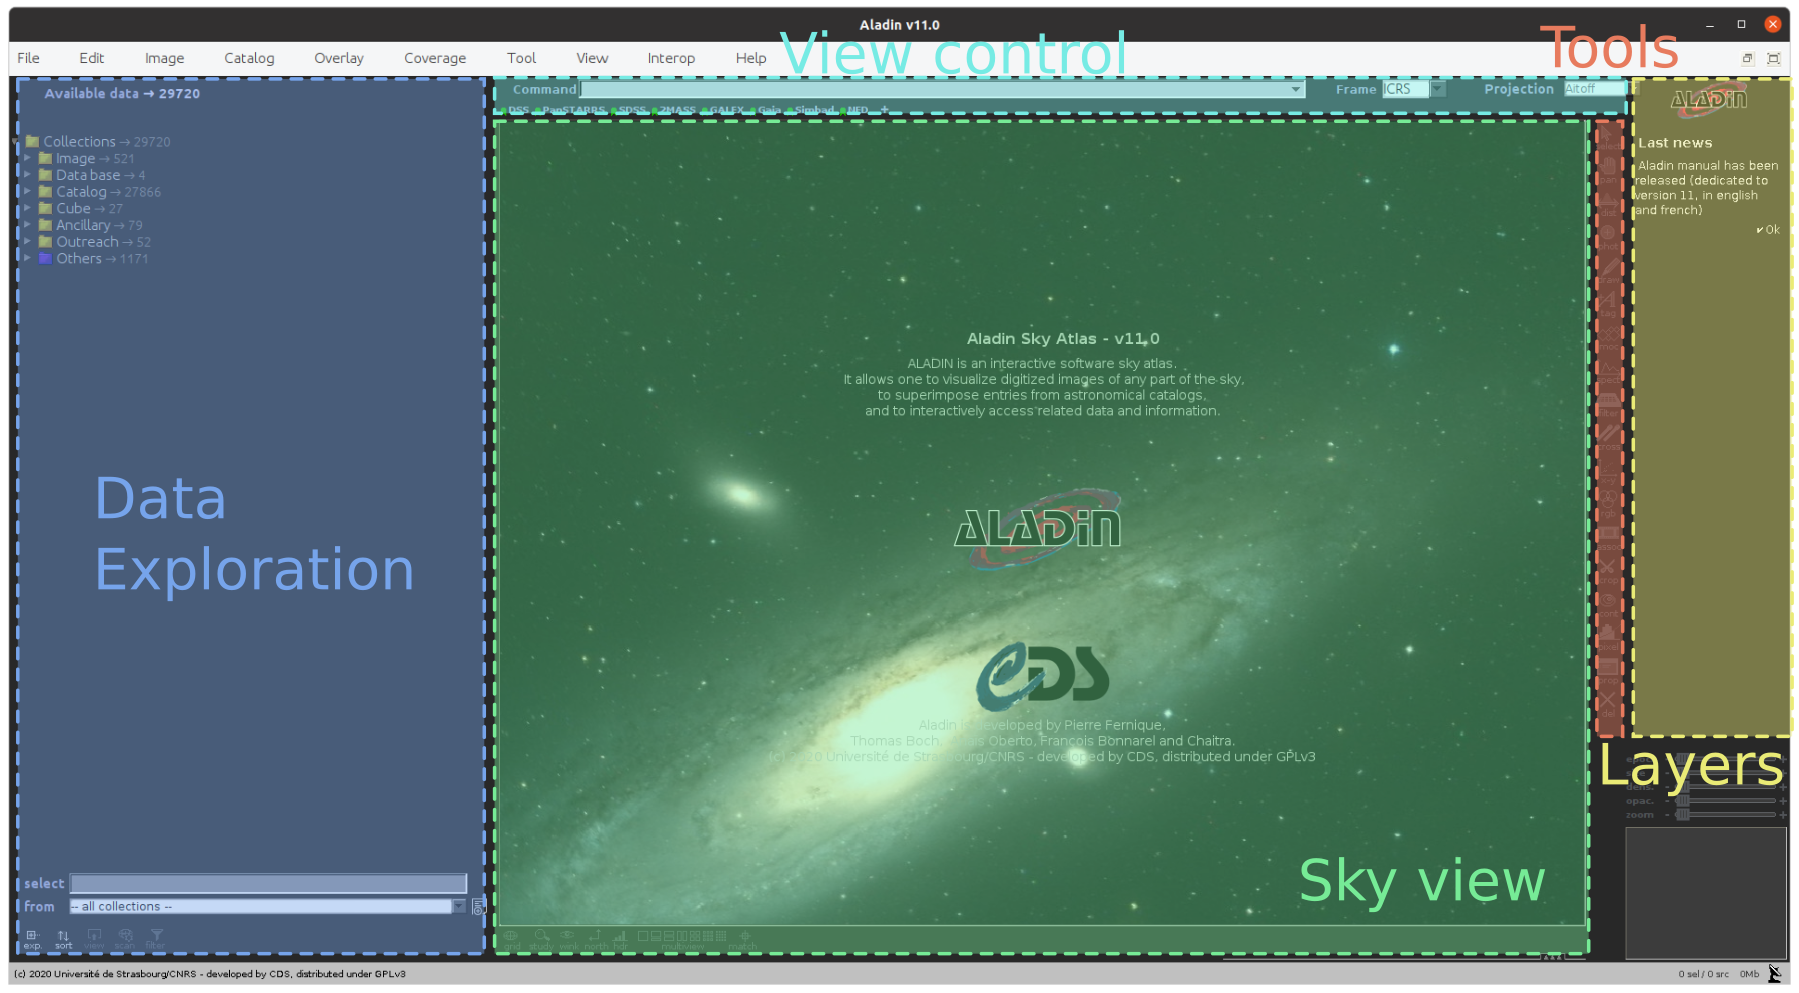
\includegraphics[width=0.8\hsize]{aladin}
  \caption{The \aladin client. Loaded data from the
  \texttt{data exploration} panel are listed as
  \texttt{layers} and displayed in the  
  \texttt{sky view}. Coordinates can be entered in the
  \texttt{view control} panel, and many
  \texttt{tools} are available.
  }
  \label{fig:aladin}
\end{figure}
%%%--------------------------------------------------------------------------------

\newpage
  \begin{enumerate}
    \setlength\itemsep{0em}
    \item Launch \aladin.
    \item Using the \texttt{View Control} (see Fig. \ref{fig:aladin}), center de view on 
          RA = $07^{h}\,08^{m}$, DEC = $+26^{\circ}\,34^{m}$ \reftips{1}
	\item Using the \texttt{Data Exploration}, open the \skybot interface \reftips{2}
  \end{enumerate}
  \setcounter{saveitem}{\value{enumi}}  

%%%--------------------------------------------------------------------------------
\begin{wrapfigure}[11]{r}{0.4\textwidth}
  \vspace{-2.5em}
  \begin{center}
    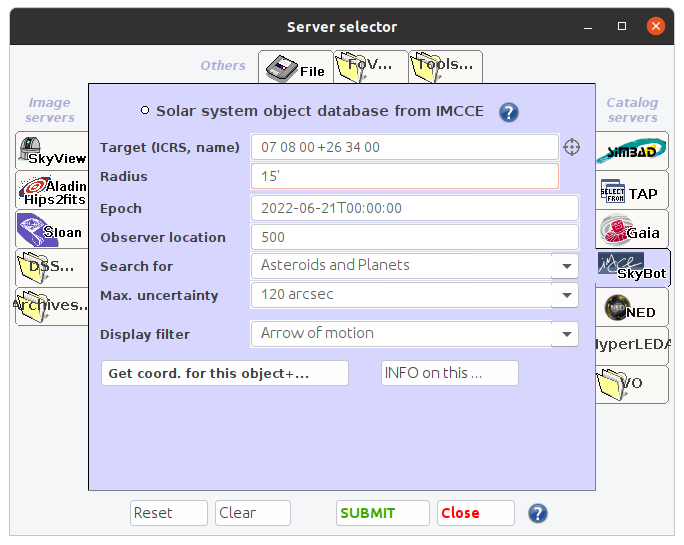
\includegraphics[width=\hsize]{skybot-server_selector}
  \end{center}
\end{wrapfigure}
%%%--------------------------------------------------------------------------------

  There are seven fieds in the pop-up window:
  \texttt{Target},
  \texttt{Radius},
  \texttt{Epoch},
  \texttt{Observer location},
  \texttt{Search For},
  \texttt{Max. uncertainty}, and
  \texttt{Display filter}.
  By default, \aladin fills the
  \texttt{Target} and
  \texttt{Radius} fields to correspond to current display.

  \begin{enumerate}
    \setlength\itemsep{0em}
    \setcounter{enumi}{\value{saveitem}}
    \item Check that the coordinates in \texttt{Target} correspond to the value above.

    \item Set the \texttt{Radius} to \texttt{15'}.

    \item Set the \texttt{Epoch} to \texttt{2022-06-21T00:00:00}.

    \item Let everything else by default and click on \texttt{SUBMIT}.
  \end{enumerate}
  \setcounter{saveitem}{\value{enumi}}  

  A new layer has appeared, showing the SSOs with their
  arrow of motion. Like for any other catalog loaded in \aladin,
  you can select objects and see their properties in the bottom panel.

  \begin{enumerate}
    \setlength\itemsep{0em}
    \setcounter{enumi}{\value{saveitem}}
    \item Select all SSOs. \texttt{Ctrl-A} or \texttt{Edit} $\rightarrow$ \texttt{Select all objects}.
    \item Flyover any of the column in the bottom panel. An histogram of values for all objects will 
          appear at the bottom right (except for columns \texttt{Name}, \texttt{RA} and \texttt{DEC}).
    \item Flyover the \texttt{Class} column then flyover the histogram to see the corresponding 
          targets in the FoV.
  \end{enumerate}

  \setcounter{saveitem}{\value{enumi}}  

  We just used a \textbf{tiny} fraction of what \aladin can do.
  With it, you can retrieve catalogs, images, cross-match them,
  select intersections, unions, etc. It is an extremely powerful
  tool to explore the sky.

\subsection*{Tips}

\begin{itemize}[label=]
	\item \tips{[1]}{enter the string "07 08 +26 34" in the Command field}
	\item \tips{[2]}{enter "skybot" in the select field, wait a couple of seconds then select
		Sky Body Tracker in the list of collections and finally Load. Alternatively, open the 
		Server selector (File $\rightarrow$ Open server selector, shortcut Ctrl-L) and select
		\skybot in the Catalog servers (right tab).}
\end{itemize}




\section{In a script}

We often process many images. Clicking on a GUI is not the most
productive method. We thus often write scripts to perform
many automated steps. Most VO services can be called through APIs
and be scripted.\\

Generally, the service has a base \texttt{url} to which queries are
to be sent. The user choices are submitted through a list of \texttt{parameter}=\texttt{value}
arguments. Of course, we cannot guess which \texttt{parameter} is
available, nor what \texttt{value} are allowed. So read the documentation!\\

For instance, we can repeat the query above in \python (see \texttt{scripts/query\_skybot.py}):

\begin{lstlisting}[language=python]
import requests
import json
import pandas as pd
from astropy.coordinates import Angle

# User choices
ep = '2022-06-21T00:00:00'
ra = '07h08m00'
dec = '+26d34m00'
sr = 15/60
observer = '500'

# Service URL
url = 'https://ssp.imcce.fr/webservices/skybot/api/conesearch.php?'

# Query parameters
params = {
     '-ep': ep,
     '-ra': Angle(ra).degree,
     '-dec': Angle(dec).degree,
     '-sr': sr,
     '-mime': 'text',
     '-output': 'all',
     '-loc': observer, 
     '-tscale': 'UTC'
    }

# Query the service
r = requests.post(url, params=params, timeout=2000)

# Write results to disc
with open("response.txt", "w") as f:
    f.write(r.text)

# Load results in a pandas.DataFrame
data = pd.read_csv( 'response.txt', sep='|', skiprows=2 )
\end{lstlisting}

So long story short, we first define the parameters (coordinates, radius, epoch) then query the
\skybot service thanks to the \texttt{request} package. The results
are written in a file, and read as a \texttt{pandas} \texttt{DataFrame}.
Performing this query for each image acquired by a telescope is very easy
(the parameters are contained in the image).\\

The script above is a simple example, let's move to the notebook
\texttt{3.3.2-How\_to\_query\_an\_API.ipynb} in the directory 
\texttt{3.2-Query\_APIs} to get some practice.



%%%--- Bibliography ---%%%
  \bibliographystyle{aa} 
  \bibliography{main}

\end{document}
